\documentclass[aspectratio=169]{beamer} % 使用16:9宽屏比例

% 使用 Moloch 主题（metropolis 的更新分支）
\usetheme{moloch}

\usepackage{fontspec}
% 设置无衬线字体（slides 主要使用无衬线字体）为 Times New Roman
\setsansfont{Times New Roman}

% --- 中文支持与主题设置 ---
\usepackage{ctex}          % 引入 ctex 宏包以支持中文

\usepackage{amsmath}

% --- 文稿基本信息 ---
\title{近地航行与控制}
\author{金承果~张洮瑞~姜世骥~张钊源}
\institute{}

\begin{document}
	
	% 标题页
	\begin{frame}
		\titlepage
	\end{frame}
	
	% Page1 齐奥尔科夫斯基方程
	\begin{frame}{Циолковский Equation}
		设发动机喷出工质相对箭体的速度为$v_e$，在任一时间刻列写动量守恒：
		$$
		mv = (m+dm)(v+dv) + (-dm)(v-v_e)
		$$
		展开并忽略高阶无穷小项：
		$$
		mdv + v_e dm = 0
		$$
		积分得到代数形式：
		$$
		\Delta v = v_e \ln \frac{m_0}{m_f}
		$$
		其中$m_0$是火箭总质量，$m_f$是火箭干重。该方程称为齐奥尔科夫斯基方程(Циолковский Equation)，给出了目标$\Delta v$下的最小质量比。
	\end{frame}
	
	% Page2 动力学ODE模型
	\begin{frame}{Dynamic Model}
		二维极坐标下，考虑万有引力与空气阻力时，模型的动力学方程如下：
		$$
		\begin{cases}
			\dot{r} = u \\
			\dot{\theta} = \frac{w}{r} \\
			\dot{u} = \frac{w^2}{r} + \frac{cq\cos\alpha}{m} - \frac{\mu}{r^2} - \frac{k(h)Vu}{m} \\
			\dot{w} = -\frac{uw}{r} + \frac{cq\sin\alpha}{m} - \frac{k(h)Vw}{m} \\
			\dot{m} = -q
		\end{cases}
		$$
		其中$\mu = GM$，作为引力项的系数；\\
		空气阻力项使用平方模型，大气使用指数密度模型：
		$$
		\begin{cases}
			f = k(h)v^2 \\
			k(h) = \frac{1}{2}\rho(h) C A \\
			\rho(h) = \rho_0 e^{-\frac{h}{H}}
		\end{cases}
		$$
		
	\end{frame}
	
	% Page3 RK4
	\begin{frame}{Numerical Solution and Runge-Kutta Method}
		使用四阶龙格-库塔法(Runge-Kutta Method)解常微分方程数值解。\\
		对于初值问题$\dot{y} = f(t,y),~~y(t_0) = y_0$，对于时刻$n$，取四个试探点：
		$$
		k_1 = f(t_n,y_n)
		$$
		$$
		k_2 = f(t_n+\frac{h}{2},y_n+\frac{h}{2}k_1)
		$$
		$$
		k_3 = f(t_n+\frac{h}{2},y_n+\frac{h}{2}k_2)
		$$
		$$
		k_4 = f(t_n+h,y_n+h k_3)
		$$
		更新下一时刻：
		$$
		y_{n+1} = y_n + \frac{h}{6}(k_1+2k_2+2k_3+k_4)
		$$
		其中$h$是可以选择的超参数，用于控制仿真精度。
	\end{frame}
	
	% Page4 PSO
	\begin{frame}{Trajectory Planning and Particle Swarm Optimization}
		粒子群算法(Particle Swarm Optimization)优化原理如下：
		$$
		\begin{cases}
			v_i^{t+1} = w v_i^t + c_1r_1(p^t_i-x^t_i) + c_2r_2(g^t_i-x^t_i) \\
			x_i^{t+1} = x_i^t + v_i^{t+1}
		\end{cases}
		$$
		其中$w$为惯性系数、$c_1$为个体学习系数、$c_2$为群体学习系数；\\
		使用的损失函数$J_{\mathrm{orbit}}=\left(\frac{h_f-h_*}{10000(\mathrm m)}\right)^2+\left(\frac{u_f}{1000(\mathrm{m/s})}\right)^2+\left(\frac{w_f-v_c}{1000(\mathrm{m/s})}\right)^2$\\
		特别地，如果燃料不足以完成规划任务，损失为$J=1000+\left(\frac{M_{\mathrm{used}}-(m_0-m_{\mathrm{dry}})}{1000,\mathrm{kg}}\right)^2$\\
		如果规划任务中火箭坠毁落地，损失为$J=J_{\mathrm{orbit}}+100+\frac{t_f-t_{\mathrm{impact}}}{1,\mathrm s}$
		
	\end{frame}
	
	% Page 5 工程启发
	\begin{frame}{Trajectory Planning and Particle Swarm Optimization}
		优化控制量为喷气攻角$\delta(t)$和燃烧速率$q(t)$；原问题在$C^{\infty}$无穷维空间上搜索。\\
		采用亚轨道燃烧-滑行入轨-圆轨燃烧的工程结构，将两个函数限制为分段阶梯函数，问题退化到有限维空间中的求解。
		$$
		z = [\delta_1, \cdots, \delta_n, q_1, q_2, t_1, t_c, t_2]
		$$
		PSO优化完成后，将最优结果的状态空间轨迹存储，作为后续控制的参考目标。
	\end{frame}
	
	% Page 6 MPC
	\begin{frame}{Model Predict Control}
		模型预测控制(MPC)是一种控制算法，主要用于白盒系统的控制。使用的优化损失函数包含状态误差、控制幅度、控制变化、松弛惩罚：
		$$
		J_{MPC} = \sum_{j=1}^N e_{k+j|k}^T Q_j e_{k+j|k} + \sum_{j=0}^{N-1} v_{k+j|k}^T R v_{k+j|k} + \sum_{j=0}^{N-1} \Delta v_{k+j|k}^T R_{\Delta} \Delta v_{k+j|k} + \lambda_\epsilon \sum_{j=1}^{N} \epsilon_j^2
		$$
		其本质是对未来$N$个时间单位内进行优化，使得状态误差、控制力度等最小。执行的优化是一个二次规划问题(Quadratic Planning)，可以直接使用MATLAB内置的求解工具求解。
		
		MPC在完成优化后，只执行下一个时刻的控制量$v_{k+1}$，随后将优化窗口向后移一个时间步，重新进行优化。
		   
	\end{frame}
	
	% Page 7 结果
	\begin{frame}{The Outcome of the Project}
		\begin{figure}[htbp]
		\centering
		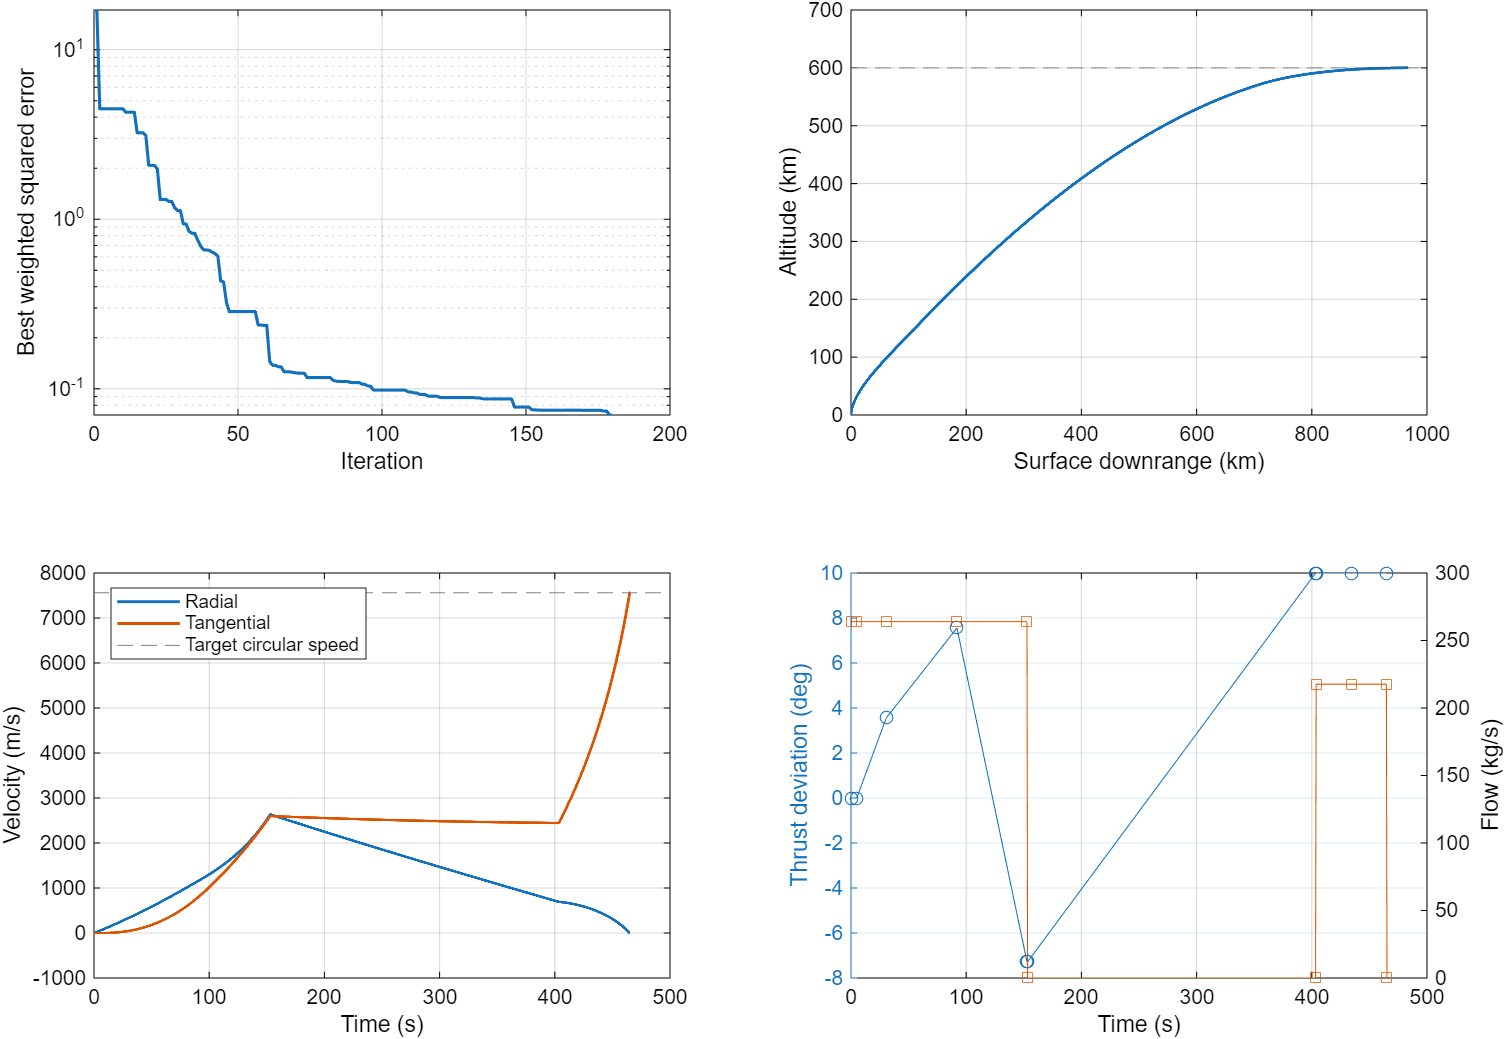
\includegraphics[width=0.7\textwidth]{fig/fig1}
		\caption{PSO规划}
		\end{figure}
	\end{frame}
	
	% Page 8 结果
	\begin{frame}{The Outcome of the Project}
		\begin{figure}[htbp]
			\centering
			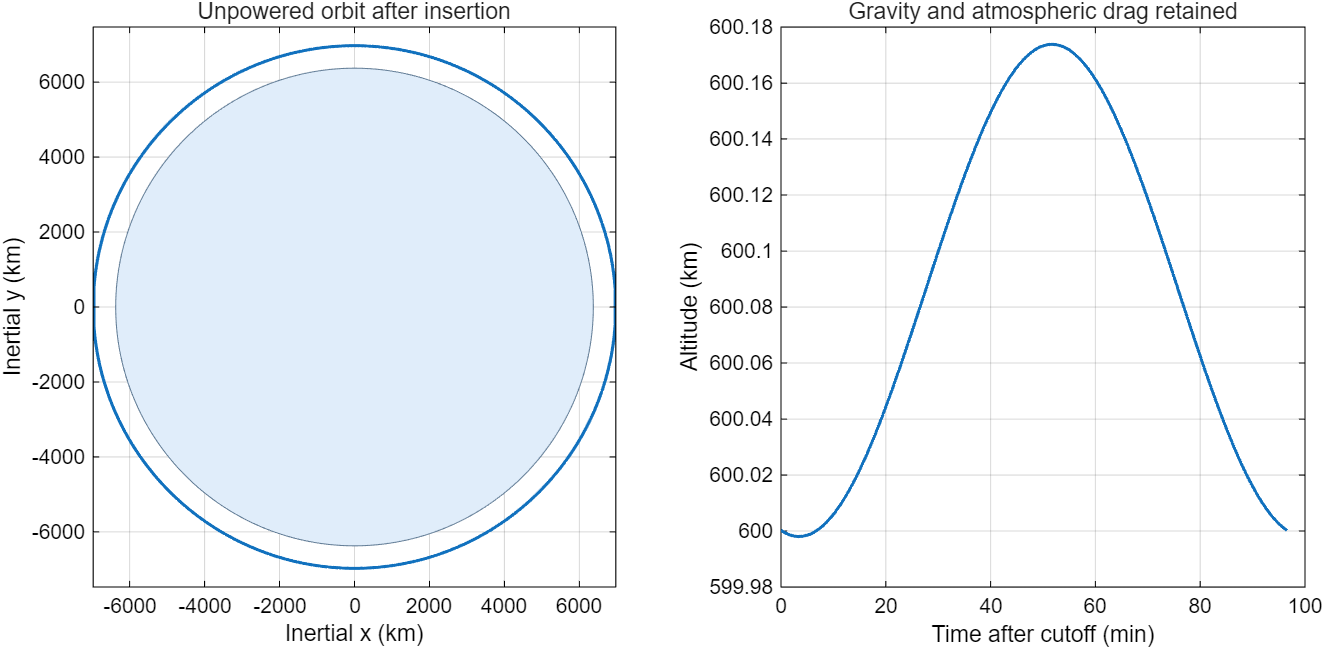
\includegraphics[width=0.7\textwidth]{fig/fig2}
			\caption{MPC控制效果}
		\end{figure}
	\end{frame}
	
\end{document}